\documentclass{article}
\usepackage{graphicx} % Required for inserting images

\title{\textbf{Transtorno del Espectro Autista}}
\author{Integrantes: Victoria García Lovelle\\
Lydia Ortiz Hernández\\
Lucía Gonzalez Redondo\\ 
María García Paredes}
\date{May 2026}


\begin{document}

\maketitle
\newpage
\tableofcontents
\listoffigures


\newpage
El presente trabajo se basa en la revisión de diversas fuentes teóricas y documentales relevantes sobre el Trastorno del Espectro del Autismo (TEA), con el objetivo de ofrecer una visión actualizada y rigurosa sobre este trastorno del neurodesarrollo.\\

Entre las principales fuentes utilizadas destacan el manual diagnóstico DSM-5, considerado un referente internacional en la clasificación de los trastornos mentales, así como el programa bbMiradas HUBU, centrado en la detección e intervención temprana del TEA.\\

Asimismo, se han utilizado materiales formativos como e-EarlyCare, orientados a la especialización en atención temprana, que aporta una perspectiva práctica sobre la intervención en los primeros años de vida, asi como los recursos proporcionados por la Confederación Autismo España, entidad de referencia en la divulgación y apoyo a las personas con TEA y sus familias.\\

La integración de estas fuentes ha permitido abordar el TEA desde una perspectiva amplia, que incluye aspectos teóricos y diagnósticos, así como una visión centrada en la persona y su entorno.\\


\section{\textbf{Introducción al Trastorno del Espectro del Autismo (TEA)}}
\subsection{\textbf{Definición del Trastorno del Espectro del Autismo}}
El Trastorno del Espectro del Autismo (TEA) se define como un conjunto heterogéneo del neurodesarrollo, de origen neurobiológico y de inicio en la infancia, que afectan principalmente a la comunicación, la interacción social, y la flexibilidad del comportamiento y del pensamiento.\\

Se denomina "espectro" debido a la gran variabilidad en su manifestación, ya que cada persona presenta diferentes necesidades y niveles de apoyo. Entre sus principales características destacan las dificultades en el reconocimiento social, la comunicación social, la compresión del entorno y la presencia de patrones repetitivos de conducta.\\

Además, pueden verse afectadas otras áreas como el lenguaje, la respuesta a estímulos sensoriales, la coordinación motora y las capacidades cognitivas.

\subsection{\textbf{Origen y naturaleza del trastorno }}
Actualmente, no se conoce con exactitud una única causa del Trastorno del Espectro del Autismo (TEA), aunque existe consenso científico en que se trata de una condición de origen principalmente genético, en la que también pueden intervenir factores ambientales que influyen en su desarrollo.\\

Durante los primeros años de estudio del autismo se plantearon diversas hipótesis sobre su origen. Entre ellas destacó la teoría que atribuía su origen a la relación entre madre e hijo. No obstante, las investigaciones posteriores han demostrado que no existe ninguna relación causal entre las actitudes o actuaciones de los padres y el desarrollo del TEA.\\

La gran variabilidad presente dentro del espectro se explica por la interacción de múltiples factores biológicos y contextuales, lo que contribuye a explicar la gran variabilidad existente dentro del espectro.\\

Además, el TEA puede aparecer asociado a otras condiciones, como la discapacidad intelectual, los trastornos del lenguaje o dificultades en la salud mental.\\

Se trata de una condición que acompaña a la persona a lo largo de toda su vida, aunque sus manifestaciones pueden variar según la etapa evolutiva y de los apoyos recibidos. En este proceso, la familia y el entorno educativo desempeñan un papel fundamental en el desarrollo y bienestar de la persona.

\subsection{\textbf{Evolución del concepto de autismo}}
El concepto de autismo ha evolucionado de forma significativa desde sus primeras descripciones, pasando de considerarse un trastorno con características concretas a entenderse como una condición con múltiples manifestaciones y diferentes niveles de apoyo.\\

Actualmente, el Manual Diagnóstico y Estadístico de los Trastornos Mentales (DSM-5) utiliza el término Trastorno del Espectro del Autismo (TEA), integrando bajo una única categoría diagnóstica la diversidad de perfiles clinicos y reflejando la amplia variabilidad existente dentro del espectro.  


\section{\textbf{Características del Trastorno del Espectro del Autismo}}
El Trastorno del Espectro del Autismo (TEA) no presenta rasgos físicos diferenciadores, sino que se manifiesta principalmente en el desarrollo cognitivo, comunicativo y conductual de cada persona. Su expresión es muy variable, en mayor o menor medida, dificultades en la comunicación e interacción social, así como la presencia de patrones de comportamiento restrictivos y repetitivos.\\

Asimismo, puede aparecer asociado a otras condiciones como discapacidad intelectual, trastornos del lenguaje o dificultades relacionadas con la salud mental.\\

Estas características hacen especialmente útil el uso de sistemas aumentativos y alternativos de comunicación (SAAC), como el uso de pictogramas, que facilitan la comprensión, la anticipación y la expresión del lenguaje.

\subsection{\textbf{Alteraciones en la comunicación e interacción social}}
Las dificultades en la comunicación y la interacción social constituyen una de las principales características del TEA. Las personas con este trastorno pueden presentar limitaciones en la reciprocidad social y emocional, lo que dificulta la comprensión de normas sociales implícitas y afecta a sus relaciones interpersonales.\\

Entre las principales dificultades destacan la comprensión de mensajes complejos como bromas, ironías, metáforas o dobles sentidos, así como la interpretación de la comunicación no verbal, incluyendo gestos, expresiones faciales y contacto visual. También pueden presentar problemas para ajustar el lenguaje al contexto comunicativo, iniciar y mantener conversaciones, comprender emociones, intenciones o pensamientos de otras personas y expresar adecuadamente sus propias emociones.\\ 

Estas limitaciones pueden generar dificultades en la participación social, el entorno escolar y el establecimiento de relaciones personales estables. 

\subsection{\textbf{Rigidez cognitiva, rutinas y patrones repetitivos}}
Las personas con TEA suelen presentar un estilo de pensamiento más rígido y dificultades para adaptarse a los cambios, lo que puede generar una fuerte necesidad de mantener rutinas y entornos predecibles. La alteración de estas rutinas o la aparición de situaciones nuevas puede provocar ansiedad, frustración o desregulación emocional.\\

Entre las manifestaciones más frecuentes se encuentran la resistencia a los cambios en el entorno o en las actividades diarias, la dificultad para anticipar situaciones nuevas, la necesidad de apoyos para afrontar contextos desconocidos, la presencia de intereses restringidos o muy focalizados y la aparición de conductas repetitivas o estereotipadas.\\

Estas características justifican la importancia de utilizar apoyos visuales y herramientas estructuradas que aporten seguridad, anticipación y una mayor comprensión del entorno. 

\subsection{\textbf{Alteraciones en el procesamiento sensorial}}
Las personas con TEA pueden presentar alteraciones en el procesamiento sensorial, mostrando tanto hiperreactividad como hiporreactividad ante determinados estímulos del entorno. Esto significa que algunos sonidos, luces, olores, texturas o temperaturas pueden generar un malestar intenso o, por el contrario, pasar prácticamente desapercibidos.\\

Entre las manifestaciones más frecuentes se encuentran la sensibilidad excesiva ante determinados estímulos, el interés inusual por experiencias sensoriales concretas, la aparente indiferencia al dolor o a la temperatura y la búsqueda de estimulación mediante conductas repetitivas como balanceos, giros o saltos.\\

Estas dificultades pueden influir en el aprendizaje, la comunicación y la interacción social, por lo que resulta fundamental adaptar el entorno y utilizar apoyos que reduzcan la sobrecarga sensorial.

\subsection{\textbf{Otras características asociadas}}
Además de las características principales, el TEA puede aparecer asociado a otras condiciones que influyen en el desarrollo y en las necesidades de apoyo de cada persona. Entre las más frecuentes se encuentran las dificultades cognitivas o de aprendizaje, los trastornos del lenguaje, los problemas de salud mental y determinadas patologías médicas.\\

La presencia de estas condiciones asociadas refuerza la necesidad de una intervención individualizada y adaptada a las características específicas de cada niño o niña. 

\subsection{\textbf{Habilidades y fortalezas en personas con Trastorno del Espectro del Autismo}}
El TEA no debe entenderse únicamente desde las dificultades asociadas, sino también desde las capacidades y fortaleza que muchas personas pueden presentar. El autismo implica una forma diferente de procesar la información y de comprender el entorno, lo que puede favorecer el desarrollo de determinadas habilidades.\\

Entre las fortalezas más frecuentes destacan la meticulosidad y la atención al detalle, la sinceridad y honestidad en las relaciones interpersonales, el conocimiento profundo sobre temas específicos de interés, así como un buen desempeño en tareas rutinarias, estructuradas o repetitivas. Asimismo, muchas personas con TEA presentan un procesamiento más lógico de la información y una mayor tendencia al respeto de las normas y reglas establecidas.\\

Reconocer estas fortalezas resulta fundamental para diseñar intervenciones centradas no solo en las dificultades, sino también en el potencial y la autonomía de cada persona.


\section{\textbf{Etiología y teorías explicativas del Trastorno del Espectro del Autismo}}
\subsection{\textbf{Factores genéticos y ambientales}}
El Trastorno del Espectro del Autismo (TEA) es una condición del neurodesarrollo de origen multifactorial, en la que intervienen factores genéticos y ambientales. Existe un consenso científico generalizado en que no responde a una única causa, sino a la interacción de múltiples factores que influyen en el desarrollo neurológico temprano.\\

Desde el punto de vista genético, el TEA presenta una elevada heredabilidad y se ha relacionado con múltiples genes implicados en el desarrollo y funcionamiento del sistema nervioso central. Estas alteraciones genéticas son heterogéneas y contribuyen a la amplia variabilidad fenotípica del espectro autista.\\

En cuanto a los factores ambientales, estos cobran especial relevancia durante las etapas prenatal y perinatal, incluyendo complicaciones obstétricas, infecciones durante el embarazo o la exposición a determinados agentes ambientales que pueden influir en el desarrollo neurológico temprano.\\

Estos factores no actúan de forma aislada, sino en interacción con la predisposición genética, modulando tanto la probabilidad de aparición del trastorno como su expresión clínica. En conjunto, esta interacción explica la gran variabilidad del TEA, lo que justifica la necesidad de intervenciones individualizadas adaptadas a cada persona.

\subsection{\textbf{Teorías explicativas del Trastorno del Espectro del Autismo}}
Se han propuesto diversas teorías con el objetivo de explicar los procesos cognitivos subyacentes al TEA, las cuales permiten comprender diferentes dimensiones de su manifestación clínica.\\

Entre las principales teorías destacan las siguientes:
\begin{itemize}
    \item \textbf{Teoría de la mente}: hace referencia a la dificultad para inferir, representar y comprender los estados mentales, intenciones y creencias de otras personas. 
    \item \textbf{Déficit en las funciones ejecutivas}: implican alteraciones en procesos como la autorregulación, la planificación, la toma de decisiones, la resolución de problemas y el control inhibitorio.
    \item \textbf{Débil coherencia central}: se caracteriza por una tendencia a procesar la información de forma fragmentada, con dificultades para integrar el contexto y extraer el significado global.
    \item \textbf{Estilos de procesamiento de la información}: como una preferencia por el procesamiento local o detallado, más que un déficit cognitivo global.
    \item \textbf{Alteraciones en la intersubjetividad}: relacionadas con dificultades en el reconocimiento, procesamiento y regulación de las emociones en la interacción social.
    \item \textbf{Déficit en atención conjunta}: se refiere a limitaciones en la capacidad de compartir la atención y estados afectivos con otras personas.
\end{itemize}

Aunque estas teorías aportan explicaciones complementarias sobre distintos aspectos del TEA, ninguna de ellas resulta suficiente de manera aislada para explicar la totalidad del trastorno. El TEA debe entenderse desde una perspectiva multidimensional, en la que las alteraciones cognitivas interactúan con factores contextuales y del desarrollo.\\

Por ello, resulta necesario adoptar un enfoque integral a lo largo del ciclo vital, considerando variables como el género, la presencia de comorbilidades y el contexto familiar y sociocultural. Esta comprensión global no solo permite entender mejor el funcionamiento de las personas con TEA, sino que también orienta el diseño de intervenciones adaptadas, centradas tanto en las dificultades como en el impacto funcional en la vida diaria. En este sentido, la utilización de apoyos visuales y sistemas aumentativos de comunicación contribuye a mejorar la comprensión del entorno y la interacción social. 


\section{\textbf{Clasificación y diagnóstico del Trastorno del Espectro del Autismo}}
\subsection{\textbf{Clasificación según CIE-11}}
La Clasificación Internacional de Enfermedades (CIE-11), elaborado por la Organización Mundial de la Salud (OMS), incluye el TEA dentro de los trastornos del neurodesarrollo, destacando su carácter dimensional y la gran variabilidad en su presentación.\\

En lugar de considerar el TEA como categorías separadas, la CIE-11 lo entiende como un espectro único en el que cada persona puede presentar diferentes niveles de afectación y necesidades de apoyo. Entre los aspectos que se tienen en cuenta para describir el perfil individual se incluyen la presencia o ausencia de discapacidad intelectual, las alteraciones del lenguaje funcional y el grado de autonomía en la vida diaria.\\

Esta variabilidad implica que no exista un único perfil de funcionamiento, sino múltiples formas de manifestación del trastorno, lo que requiere intervenciones adaptadas a cada caso. En este contexto, el uso de sistemas aumentativos y alternativos de comunicación, como los pictogramas, resulta especialmente relevante para favorecer la comprensión del entorno y facilitar la comunicación en distintos niveles de funcionamiento.

\subsection{\textbf{Criterios diagnósticos según DSM-5}}
El diagnóstico del Trastorno del Espectro del Autismo (TEA), según el DSM-5, se basa en la presencia de dificultades persistentes en la comunicación e interacción social, así como en patrones restrictivos y repetitivos de comportamiento, intereses o actividades. Estos síntomas deben aparecer en las primeras etapas del desarrollo y producir un impacto significativo en el funcionamiento diario de la persona.\\

En el ámbito de la comunicación e interacción social, se incluyen dificultades en la reciprocidad socioemocional, en la comunicación verbal y no verbal (como el uso del contacto visual, gestos o expresión facial) y en el desarrollo y mantenimiento de relaciones sociales.\\

Por otro lado, los patrones restrictivos y repetitivos pueden manifestarse mediante conductas estereotipadas, rigidez ante los cambios, intereses altamente focalizados y alteraciones en el procesamiento sensorial, como hiperreactividad o hiporreactividad a determinados estímulos.\\

Los síntomas deben presentarse desde el desarrollo temprano y generar un impacto funcional en la vida social, educativa o personal. Asimismo, es necesario descartar que estas dificultades se expliquen mejor por otras condiciones del desarrollo, aunque pueden coexistir con discapacidad intelectual u otras alteraciones.\\

Estos criterios permiten una comprensión estructurada del TEA y refuerzan la necesidad de intervenciones adaptadas, como el uso de sistemas aumentativos y alternativos de comunicación, que faciliten la comprensión del entorno y la expresión funcional en distintos contextos.

\clearpage
\subsection{\textbf{Niveles de gravedad del Trastorno del Espectro del Autismo}}
\begin{figure}[!htbp]
\centering
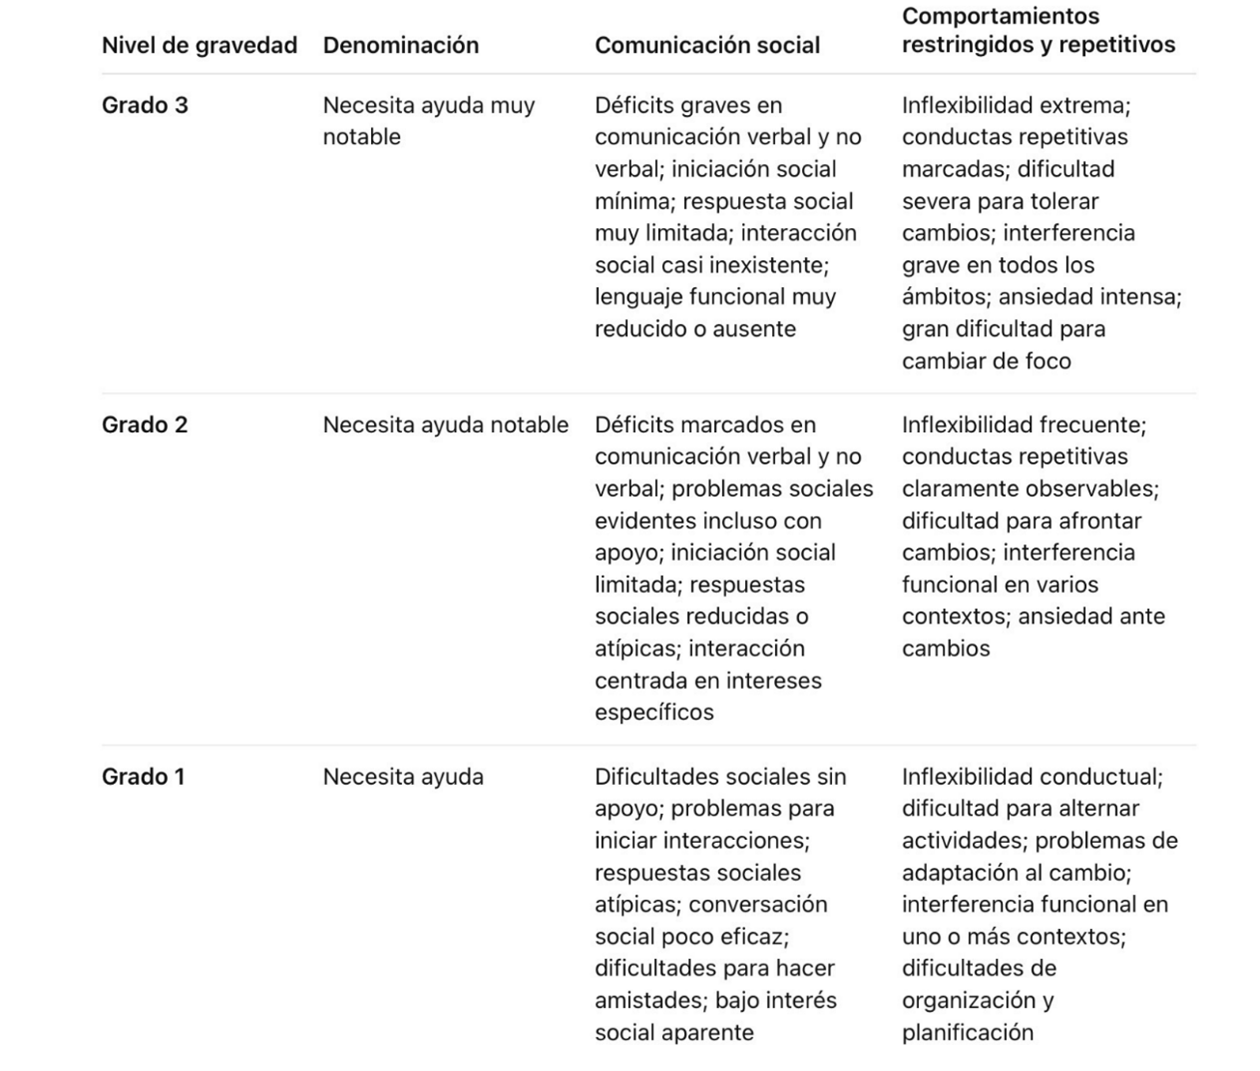
\includegraphics[width=0.7\textwidth]{Imagen1.png}
\caption{Niveles de gravedad del trastorno del espectro del autismo según DSM-5.}
\end{figure}


\section{\textbf{Prevalencia del Trastorno del Espectro del Autismo}}
\subsection{\textbf{Datos de prevalencia en Europa}}
En Europa, la prevalencia del Trastorno del Espectro del Autismo (TEA) se sitúa aproximadamente en torno a 1 de cada 100 personas, aunque estas cifras pueden variar en función de los criterios diagnósticos utilizados, los métodos de recogida de datos y el acceso a los servicios de evaluación en cada país.\\

Los estudios epidemiológicos recientes reflejan variaciones entre países europeos, con estimaciones ligeramente superiores en aquellos con sistemas de detección más desarrollados, y valores algo inferiores en regiones con menor acceso a recursos diagnósticos. Esta variabilidad no implica necesariamente diferencias reales en la prevalencia, sino que está influida por factores como la conciencia social sobre el TEA, la disponibilidad de servicios especializados y la organización de los sistemas sanitarios.\\

En conjunto, estos datos ponen de manifiesto la importancia del diagnóstico temprano y del acceso equitativo a herramientas de apoyo, especialmente en el ámbito educativo y comunicativo.

\clearpage
\subsection{\textbf{Datos de prevalencia en España}}
\begin{figure}[!htbp]
\centering
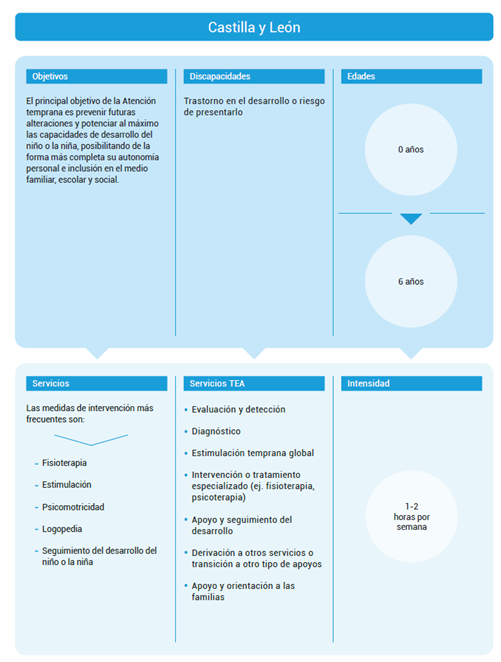
\includegraphics[width=0.7\textwidth]{Imagen2.png}
\caption{Situación de la atención temprana de TEA en Castilla y León.}
\end{figure}
\clearpage

En España, los datos de prevalencia del Trastorno del Espectro del Autismo (TEA) son similares a los del resto de Europa, estimándose que aproximadamente 1 de cada 100 personas presenta esta condición.\\

Teniendo en cuenta la población española actual, se calcula que el número de personas con TEA se sitúa en torno a las 500.000, lo que pone de manifiesto la relevancia social y sanitaria de este trastorno, así como la necesidad de desarrollar recursos de apoyo adecuados.\\

Además, debido a la distribución competencial del sistema sanitario y educativo en España, las comunidades autónomas son las encargadas de organizar y gestionar los servicios de atención temprana. Esta descentralización puede dar lugar a variaciones en los recursos disponibles, lo que se traduce en posibles desigualdades en el acceso a la intervención en función del territorio.\\

En este contexto, el desarrollo de herramientas digitales accesibles, como aplicaciones basadas en pictogramas, puede contribuir a reducir estas barreras y facilitar la comunicación en distintos entornos.

\subsection{\textbf{Variabilidad según factores individuales}}

La detección y el diagnóstico del Trastorno del Espectro del Autismo (TEA) pueden variar en función de diferentes factores individuales y contextuales, lo que contribuye a la heterogeneidad en la identificación del trastorno.\\

En relación con el género, se ha observado que las niñas con TEA suelen recibir un diagnóstico más tardío que los niños. Esto se debe, en parte, a diferencias en la expresión de los síntomas y al uso de estrategias de camuflaje social, mediante las cuales pueden enmascarar sus dificultades para adaptarse a las demandas del entorno.\\

Asimismo, la edad de diagnóstico en Europa se sitúa de media entre los 36 y 46 meses, aunque en muchos casos la identificación se produce más tarde, especialmente en perfiles con menor afectación funcional. Esto puede retrasar el acceso a intervenciones tempranas, fundamentales para el desarrollo de habilidades comunicativas y sociales.\\

La gravedad de los síntomas también influye en la detección, ya que los casos con mayor necesidad de apoyo suelen identificarse antes, mientras que los perfiles más leves pueden pasar desapercibidos durante más tiempo.\\

Finalmente, factores socioeconómicos, culturales y educativos desempeñan un papel relevante en el acceso a los servicios diagnósticos, contribuyendo a la variabilidad observada tanto entre regiones como dentro de un mismo país. En este contexto, la detección temprana y el acceso a herramientas de apoyo comunicativo resultan esenciales para mejorar la intervención en edades tempranas.


\section{\textbf{Detección temprana del Trastorno del Espectro del Autismo}}
\subsection{\textbf{Importancia de la detección precoz}}
La detección temprana del Trastorno del Espectro del Autismo (TEA) es clave para favorecer un desarrollo óptimo y mejorar el pronóstico a largo plazo. Identificar signos de riesgo en los primeros años de vida permite iniciar intervenciones ajustadas a las necesidades del niño o niña, lo que influye de forma significativa en su evolución.\\

La intervención precoz facilita el desarrollo de habilidades sociales, comunicativas y cognitivas, además de reducir el impacto de dificultades asociadas como problemas de aprendizaje, ansiedad o alteraciones del sueño. Asimismo, permite una mejor planificación del entorno familiar y educativo desde etapas iniciales. Se ha demostrado que la intervención antes de los 3 años aprovecha la mayor plasticidad cerebral, favoreciendo la adquisición de aprendizajes y la autonomía funcional.\\

No obstante, la detección temprana no siempre implica un diagnóstico inmediato, especialmente en casos con menor afectación funcional, donde los síntomas pueden ser más sutiles o confundirse con otros trastornos del desarrollo. Además, en niñas puede existir infradiagnóstico debido a estrategias de camuflaje social, lo que puede retrasar el acceso a apoyos adecuados.\\

En este contexto, resulta fundamental disponer de herramientas accesibles que faciliten la comunicación y la comprensión del entorno desde edades tempranas, como los sistemas aumentativos de comunicación basados en pictogramas, que constituyen el eje principal de este trabajo.

\subsection{\textbf{Signos de alerta en el desarrollo infantil}}
Los signos de alerta varían según la edad del niño y afectan principalmente la comunicación, la interacción social y el comportamiento. Estos signos no son diagnósticos por sí mismos, pero sirven como indicadores que justifican una evaluación profesional especializada. La Confederación Autismo España los clasifica de la siguiente manera:

\begin{figure}[!htbp]
\centering
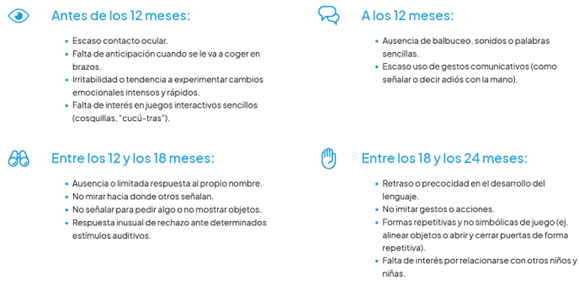
\includegraphics[width=0.7\textwidth]{Imagen3.png}
\caption{Clasificación de los signos de alerta según la Confederación Autismo España.}
\end{figure}
 
\FloatBarrier

\subsection{\textbf{Instrumentos de cribado y detección}}
\begin{figure}[!htbp]
\centering
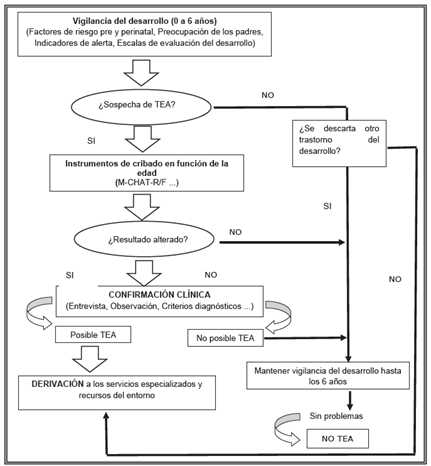
\includegraphics[width=\textwidth]{Imagen4.png}
\caption{Algoritmo de decisión para la detección del TEA.}
\end{figure} 

\FloatBarrier

Existen diversas herramientas estandarizadas que combinan observación clínica, cuestionarios y escalas estructuradas con el objetivo de identificar posibles signos de Trastorno del Espectro del Autismo (TEA) en etapas tempranas.\\

Entre los principales instrumentos de cribado destacan cuestionarios dirigidos a familias, como el M-CHAT y su versión revisada M-CHAT-R/F, diseñados para evaluar el riesgo de TEA en edades tempranas. Otros ejemplos incluyen el PDDST-II, el ESAT o el SCQ, este último indicado a partir de los 4 años y centrado en la evaluación de la comunicación social y conductas restrictivas. Asimismo, la escala Haizea-Llevant, validada en España, permite valorar el desarrollo infantil entre el nacimiento y los 5 años, detectando posibles desviaciones en el desarrollo evolutivo.\\

En cuanto al diagnóstico clínico, este requiere un enfoque multidisciplinar que incluye evaluación médica y neurológica, análisis del desarrollo y colaboración de profesionales especializados como psicólogos, logopedas y pediatras. Dentro de este proceso destacan herramientas estructuradas como la entrevista ADI-R, dirigida a familias, y la observación estandarizada ADOS-2, centrada en la interacción social y la comunicación.\\

Estas herramientas deben ser aplicadas por profesionales formados, garantizando la fiabilidad del diagnóstico y permitiendo diferenciar el TEA de otros trastornos del neurodesarrollo con sintomatología similar. La detección resulta especialmente compleja en casos leves, donde los signos pueden pasar desapercibidos y retrasar el diagnóstico, a veces hasta la etapa escolar.\\

En conjunto, la combinación de observación clínica, entrevistas y herramientas de cribado permite una identificación más precisa del riesgo de TEA, facilitando una derivación temprana a servicios especializados.


\section{\textbf{Intervención temprana en el Trastorno del Espectro del Autismo}}
\subsection{\textbf{Importancia de la intervención precoz}}
Actualmente no existe un tratamiento médico que elimine las características nucleares del Trastorno del Espectro del Autismo (TEA). Por ello, la detección e intervención tempranas son fundamentales, ya que se asocian con una mejora significativa en el desarrollo comunicativo, social y funcional de los niños y niñas.\\

La intervención precoz contribuye a aprovechar la mayor plasticidad cerebral en los primeros años de vida, facilitando la adquisición de habilidades cognitivas, sociales y comunicativas. Además, permite reducir la aparición de dificultades secundarias como problemas de conducta, ansiedad o retrasos en el rendimiento académico, al mismo tiempo que facilita la adaptación del entorno familiar y educativo a las necesidades del menor.

\subsection{\textbf{Principios de la intervención}}
La intervención temprana en el TEA debe basarse en una serie de principios fundamentales que garanticen su eficacia y adecuación a las necesidades individuales. Entre ellos destacan el inicio temprano tras la detección de signos de alerta, la individualización de las estrategias de intervención y la continuidad en distintos contextos de la vida del niño, como el entorno familiar y educativo.\\

Asimismo, resulta esencial la coordinación multidisciplinar entre profesionales como psicólogos, logopedas, terapeutas ocupacionales y pediatras, junto con la participación activa de la familia, que desempeña un papel clave en la planificación y generalización de los aprendizajes. Por último, la intervención debe desarrollarse preferentemente en entornos naturales y significativos, favoreciendo así la aplicación funcional de las habilidades adquiridas en la vida cotidiana.

\subsection{\textbf{Programas de intervención}}
Los programas de intervención en el TEA se centran en distintas áreas del desarrollo y cuentan con un respaldo creciente de la evidencia científica. Entre ellos destacan los programas orientados a la comunicación, que incluyen el uso de Sistemas Aumentativos y Alternativos de Comunicación (SAAC), así como los programas de desarrollo social, centrados en la mejora de la interacción, el juego simbólico y la atención compartida.\\

También se emplean modelos como TEACCH, que estructuran el entorno para favorecer la comprensión y la autonomía, y el Apoyo Conductual Positivo (PBS), orientado a comprender la función de las conductas problemáticas para intervenir de forma preventiva y educativa. Asimismo, las intervenciones basadas en la estimulación e integración sensorial buscan mejorar la autorregulación y la adaptación a los estímulos del entorno.


\section{\textbf{Atención temprana y apoyos a lo largo del ciclo vital}}
\subsection{\textbf{Enfoque psicoeducativo}}
La atención a las personas con Trastorno del Espectro del Autismo (TEA) se fundamenta principalmente en enfoques psicoeducativos, los cuales han demostrado una mayor eficacia en la mejora del desarrollo y la calidad de vida.\\

Estos enfoques se centran en el desarrollo de habilidades socioemocionales, comunicativas, conductuales y de autonomía personal, así como en la participación activa en la vida cotidiana, el ocio y la comunidad. Asimismo, incorporan estrategias que facilitan la comprensión del entorno físico y social, favoreciendo la comunicación y la interacción con otras personas.

\subsection{\textbf{Participación familiar}}
La familia desempeña un papel fundamental en la intervención en TEA, por lo que su implicación debe ser activa, continua y coordinada con los profesionales. Su participación resulta esencial para garantizar la coherencia de las intervenciones en los distintos contextos del niño o niña, especialmente en el entorno cotidiano.\\

En este sentido, los programas de atención temprana deben ofrecer orientación sobre recursos y apoyos disponibles, facilitar la coordinación entre familia, escuela y profesionales, e implicar a la familia en la toma de decisiones y en la intervención diaria. Esta participación activa contribuye a la generalización de los aprendizajes y a una mejor adaptación del niño o niña a su entorno natural.

\subsection{\textbf{Inclusión social y calidad de vida}}
La intervención en TEA debe orientarse hacia la promoción de una vida plena e inclusiva, centrada en la persona y en el respeto a sus derechos. Este enfoque implica no solo trabajar sobre las habilidades individuales, sino también sobre la adaptación del entorno.\\

En este sentido, resulta fundamental promover la participación en la comunidad y en entornos normalizados, mejorar la calidad de vida entendida como bienestar y autonomía personal, y garantizar la igualdad de oportunidades desde un enfoque de derechos humanos. Asimismo, es necesario reducir las barreras físicas, sociales y cognitivas, favoreciendo la accesibilidad y la participación plena.\\

Este enfoque debe acompañarse de una perspectiva de ciclo vital, adaptando los apoyos a las necesidades cambiantes de cada etapa del desarrollo.

\subsection{\textbf{Intervenciones basadas en la evidencia}}
Las intervenciones dirigidas a personas con Trastorno del Espectro del Autismo deben basarse en la evidencia científica disponible, el criterio profesional y las preferencias de la persona y su familia.\\

Estos apoyos deben estar centrados en la persona, considerando sus intereses, fortalezas y necesidades individuales, y orientarse a promover la autonomía personal y la participación social. Asimismo, deben favorecer oportunidades de interacción y aprendizaje en contextos naturales, asegurando su adecuación a las distintas etapas del desarrollo, desde la infancia hasta la vida adulta.


\section{\textbf{Marco normativo y derechos de las personas con Trastornos del Espectro del Autismo}}
En España, los niños y las niñas son titulares de los derechos fundamentales reconocidos en la Constitución Española, que además establece una protección especial debido a su situación de vulnerabilidad. En este sentido, el artículo 39.4 recoge que la infancia gozará de la protección prevista en los acuerdos internacionales ratificados por el Estado, lo que integra estos tratados dentro del ordenamiento jurídico español.

\subsection{\textbf{Convención sobre los Derechos del Niño}}
La Convención sobre los Derechos del Niño, aprobada por la ONU en 1989 y ratificada por España, constituye el principal marco internacional de protección de la infancia. Este tratado supuso un cambio de paradigma al reconocer a los niños y niñas como sujetos de pleno derecho, con capacidad de participación en las decisiones que afectan a su vida.

En relación con la discapacidad, el artículo 23 establece que los niños y niñas con discapacidad deben poder disfrutar de una vida plena y digna, desarrollarse en condiciones que garanticen su bienestar, alcanzar el máximo grado de autonomía posible y participar activamente en la comunidad.

En el marco de esta Convención, la atención a la infancia con necesidades de apoyo se articula en torno a elementos clave como la detección precoz con participación de familias y profesionales, la integración de servicios de atención temprana en sistemas públicos accesibles, la coordinación entre ámbitos sanitario, educativo y social, la continuidad de los apoyos y la reducción de barreras administrativas que dificultan el acceso a los recursos.

\subsection{\textbf{Convención Internacional de los Derechos de las Personas con Discapacidad}}
La Convención sobre los Derechos de las Personas con Discapacidad (2006), ratificada por España, supone un cambio fundamental en el enfoque de la discapacidad, pasando de un modelo asistencial a un modelo basado en derechos humanos. En este contexto, se reconoce a las personas con discapacidad como titulares plenos de derechos, situando la igualdad y la no discriminación como principios básicos.

Asimismo, la Convención destaca la importancia del respeto a la evolución de las capacidades de los niños y niñas con discapacidad, así como su derecho a preservar su identidad y recibir apoyos adecuados a sus necesidades específicas.

Sus principios fundamentales incluyen el respeto a la dignidad, la autonomía individual, la inclusión plena en la sociedad, la igualdad de oportunidades, la accesibilidad universal, la igualdad entre hombres y mujeres y el reconocimiento de la discapacidad como parte de la diversidad humana.

La Convención se estructura en tres grandes bloques. El primero recoge disposiciones generales que definen su propósito: promover, proteger y asegurar el disfrute pleno de los derechos humanos en igualdad de condiciones. El segundo constituye el núcleo central, donde se desarrollan derechos fundamentales como la protección frente a la discriminación, el acceso a la educación, la salud, la vida independiente, la participación social, política y cultural, así como la protección de colectivos especialmente vulnerables como la infancia. Finalmente, el tercer bloque establece mecanismos de aplicación, seguimiento y supervisión de la Convención por parte de los Estados.

\subsection{\textbf{Estrategia sobre los derechos de las personas con discapacidad para 2021-2030}}
La Estrategia sobre los derechos de las personas con discapacidad 2021-2030, presentada por la Comisión Europea en 2021, tiene como objetivo garantizar la plena participación de las personas con discapacidad en la sociedad en condiciones de igualdad.

Esta estrategia da continuidad a la política europea previa en materia de discapacidad y se enmarca dentro del Pilar Europeo de Derechos Sociales. Sus principales líneas de actuación se orientan a promover la igualdad de oportunidades, la inclusión social y laboral, la accesibilidad universal y la participación activa en la vida política y comunitaria.

No obstante, esta estrategia no contempla medidas específicas dirigidas a la atención temprana, sino que aborda la discapacidad desde una perspectiva global y a lo largo de todo el ciclo vital.

\subsection{\textbf{Normativa española sobre atención primaria}}
El marco normativo español en materia de discapacidad se fundamenta en la Constitución Española, que establece la obligación de los poderes públicos de promover la igualdad real y efectiva, la protección de la infancia y la inclusión social de las personas con discapacidad.

En este sentido, destacan tres artículos clave: el artículo 9.2, que obliga a los poderes públicos a eliminar desigualdades y promover condiciones de igualdad efectiva; el artículo 39, que establece la protección social, económica y jurídica de la infancia y la familia como principio rector; y el artículo 49, que recoge la obligación de impulsar políticas de prevención, rehabilitación e integración de las personas con discapacidad.

Estos principios se desarrollan en el Real Decreto Legislativo 1/2013, que refuerza la protección de los menores con discapacidad, promueve la prevención de situaciones de dependencia y garantiza una atención integral adaptada a las necesidades de cada persona.

En España, la atención temprana se organiza de forma descentralizada, siendo las comunidades autónomas las responsables de su planificación y gestión. Esta estructura da lugar a diferentes modelos de intervención y recursos, lo que puede generar variabilidad en el acceso y en la calidad de los servicios en función del territorio.

\begin{figure}[!htbp]
\centering
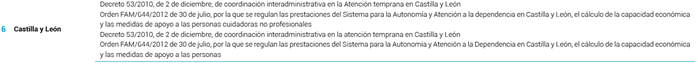
\includegraphics[width=0.7\textwidth]{Imagen5.png}
\caption{Regulación autonómica en Castilla y León.}
\end{figure}
\clearpage 


\section{\textbf{Debilidades de la atención temprana en niños y niñas con TEA en España}}
A pesar de los avances en atención temprana, en España aún existen limitaciones que afectan a la equidad, la continuidad y la accesibilidad de los servicios dirigidos a niños y niñas con Trastorno del Espectro del Autismo (TEA).\\

Una de las principales dificultades es la desigualdad entre comunidades autónomas en la organización y acceso a los recursos, lo que genera diferencias en la cobertura y calidad de la atención. A ello se suma la existencia de procedimientos administrativos complejos y una dispersión de la información, lo que puede retrasar el acceso a los servicios en una etapa en la que la intervención precoz es clave.\\

Asimismo, se observan limitaciones en la coordinación entre los ámbitos sanitario, educativo y social, así como una insuficiente continuidad en la intervención tras la etapa de atención temprana. En algunos casos, la intervención se realiza en contextos poco naturales y con una escasa implicación familiar, lo que dificulta la generalización de los aprendizajes.\\

En conjunto, estas limitaciones ponen de manifiesto la necesidad de desarrollar recursos accesibles, coordinados y centrados en la comunicación y el entorno cotidiano del niño o niña, como los sistemas aumentativos de comunicación basados en pictogramas.


\section{\textbf{Programa bbMiradas HUBU}}
El programa bbMiradas HUBU es una iniciativa orientada a la detección e intervención temprana del Trastorno del Espectro del Autismo (TEA) en la primera infancia, desarrollada por Autismo Burgos y la Fundación Miradas. Su objetivo principal es mejorar la identificación precoz de signos de riesgo mediante un seguimiento sistemático del desarrollo infantil en edades tempranas.\\

Este programa combina la evaluación clínica tradicional con el uso de tecnologías como el seguimiento ocular (eye tracking), lo que permite detectar posibles alteraciones en el desarrollo socio-comunicativo desde los primeros meses de vida.\\

En conjunto, bbMiradas pone de manifiesto la importancia de la detección temprana y del uso de herramientas innovadoras para la identificación del TEA, lo que refuerza la relevancia de desarrollar recursos de apoyo accesibles que faciliten la comunicación y la intervención desde edades tempranas.


\section{\textbf{Conclusión}}
El Trastorno del Espectro del Autismo (TEA) constituye una condición compleja del neurodesarrollo caracterizada por una gran heterogeneidad en su manifestación, lo que exige una comprensión amplia, actualizada y centrada en la persona. A lo largo de este trabajo se ha puesto de manifiesto la importancia de abordar el TEA desde un enfoque integral que contemple no solo sus características clínicas, sino también los factores etiológicos, los procesos de detección temprana y las estrategias de intervención más eficaces.\\

En este sentido, la evidencia científica destaca el valor fundamental de la detección precoz y la intervención temprana, ya que permiten potenciar el desarrollo de habilidades y mejorar la calidad de vida de las personas con TEA y sus familias. Asimismo, se evidencia la necesidad de intervenciones individualizadas, basadas en la evidencia y desarrolladas en entornos naturales, con una participación activa de la familia y una adecuada coordinación entre los distintos profesionales implicados.\\

Por otro lado, el análisis del marco normativo y de la situación actual en España pone de relieve avances significativos en el reconocimiento de derechos, pero también importantes desafíos, especialmente en relación con la equidad en el acceso a los servicios, la coordinación entre sistemas y la continuidad de los apoyos a lo largo del ciclo vital.\\

En definitiva, avanzar en el conocimiento y la intervención en el TEA implica no solo mejorar los recursos y prácticas profesionales, sino también promover una sociedad más inclusiva, que respete la diversidad, elimine barreras y garantice la igualdad de oportunidades para todas las personas.\\


\newpage
\section{\textbf{Bibliografía}}
\begin{thebibliography}{9}

\bibitem{icd11}
ICD-11 for Mortality and Morbidity Statistics. (s. f.). \url{https://icd.who.int/browse/2026-01/mms/en#437815624}

\bibitem{martinez2024}
Martínez Marín, M. Á., Escolar Llamazares, M. del C., Ortiz Huerta, J. H., Mercado Val, E., Marticorena Sánchez, R., Arnaiz González, Á., Díez Pastor, J. F., \& Rodríguez Arribas, S. (2024). \textit{Formación y especialización en atención temprana: uso de recursos tecnológicos y de inteligencia artificial} (M. C. Sáiz Manzanares \& M. Santamaría Vázquez, Eds.). UNIVERSIDAD DE BURGOS. Servicio de Publicaciones e Imagen Institucional - Libros en acceso abierto. \url{https://libros.ubu.es/servpubu-acceso-abierto/catalog/book/60}

\bibitem{dsm5}
Guía de consulta de los criterios diagnósticos del DSM-5-TR ® | México | Editorial Médica Panamericana. (s. f.). Editorial Médica Panamericana. \url{https://www.medicapanamericana.com/es-US/libros/guia-de-consulta-de-los-criterios-diagnosticos-del-dsm-5-tr}

\bibitem{moreno2020}
G. Moreno, F. Moreira, C. A. Collazos \& H. M. Fardoun, "Recommendations for the design of inclusive apps for the treatment of autism: An approach to design focused on inclusive users," \textit{2020 15th Iberian Conference on Information Systems and Technologies (CISTI)}, Seville, Spain, 2020, pp. 1-6, doi: 10.23919/CISTI49556.2020.9140816.

\bibitem{analisis_normativo}
Análisis normativo. La atención temprana que reciben los niños y las niñas con trastorno del espectro del autismo en España – SID. (s. f.). \url{https://sid-inico.usal.es/documentacion/analisis-normativo-la-atencion-temprana-que-reciben-los-ninos-y-las-ninas-con-trastorno-del-espectro-del-autismo-en-espana/}

\end{thebibliography}


\section{\textbf{Webgrafía}}
\begin{thebibliography}{9}

\bibitem{icd11}
ICD-11 for Mortality and Morbidity Statistics. (s. f.). \url{https://icd.who.int/browse/2026-01/mms/en#437815624}

\bibitem{martinez2024}
Martínez Marín, M. Á., Escolar Llamazares, M. del C., Ortiz Huerta, J. H., Mercado Val, E., Marticorena Sánchez, R., Arnaiz González, Á., Díez Pastor, J. F., \& Rodríguez Arribas, S. (2024). \textit{Formación y especialización en atención temprana: uso de recursos tecnológicos y de inteligencia artificial} (M. C. Sáiz Manzanares \& M. Santamaría Vázquez, Eds.). UNIVERSIDAD DE BURGOS. Servicio de Publicaciones e Imagen Institucional - Libros en acceso abierto. \url{https://libros.ubu.es/servpubu-acceso-abierto/catalog/book/60}

\bibitem{dsm5}
Guía de consulta de los criterios diagnósticos del DSM-5-TR ® | México | Editorial Médica Panamericana. (s. f.). Editorial Médica Panamericana. \url{https://www.medicapanamericana.com/es-US/libros/guia-de-consulta-de-los-criterios-diagnosticos-del-dsm-5-tr}

\bibitem{moreno2020}
G. Moreno, F. Moreira, C. A. Collazos \& H. M. Fardoun, "Recommendations for the design of inclusive apps for the treatment of autism: An approach to design focused on inclusive users," \textit{2020 15th Iberian Conference on Information Systems and Technologies (CISTI)}, Seville, Spain, 2020, pp. 1-6, doi: 10.23919/CISTI49556.2020.9140816.

\bibitem{analisis_normativo}
Análisis normativo. La atención temprana que reciben los niños y las niñas con trastorno del espectro del autismo en España – SID. (s. f.). \url{https://sid-inico.usal.es/documentacion/analisis-normativo-la-atencion-temprana-que-reciben-los-ninos-y-las-ninas-con-trastorno-del-espectro-del-autismo-en-espana/}

\bibitem{autismo_espana2025}
Confederación Autismo España. (2025, 9 octubre). \textit{Autismo y educación - Trastorno del Espectro Autista (TEA)}. Autismo España. \url{https://autismo.org.es/que-hacemos/lineas-de-accion/educacion/}

\bibitem{boe}
BOE.es - Agencia Estatal Boletín Oficial del Estado. (s. f.). \url{https://www.boe.es/}

\bibitem{bbmiradas_programa}
bbMiradas | Programa Detección precoz e intervención en bebés con indicadores de alerta en el desarrollo socio–comunicativo. (s. f.). \url{https://bbmiradas.fundacionmiradas.org/}

\bibitem{bbmiradas_articulo}
Adm1n1strad0r. (s. f.). \textit{Detección precoz del trastorno del espectro autista durante el primer año de vida en la consulta pediátrica | bbMiradas}. \url{https://bbmiradas.fundacionmiradas.org/download/deteccion-precoz-del-trastorno-del-espectro-autista-durante-el-primer-ano-de-vida-en-la-consulta-pediatrica}

\bibitem{ubu_biblioteca}
Biblioteca | Universidad de Burgos. (s. f.). \url{https://www.ubu.es/biblioteca}

\end{thebibliography}


\section{\textbf{Videografía}}
\begin{thebibliography}{9}

\bibitem{autismo_video2023}
Confederación Autismo España. (2023, 14 abril). \textit{¿Conoces las señales tempranas del autismo? | Detección temprana del TEA} [Vídeo]. YouTube. \url{https://www.youtube.com/watch?v=Z_Ov-M3J3Gk}

\end{thebibliography}

\end{document}


